\begin{figure}
\centering
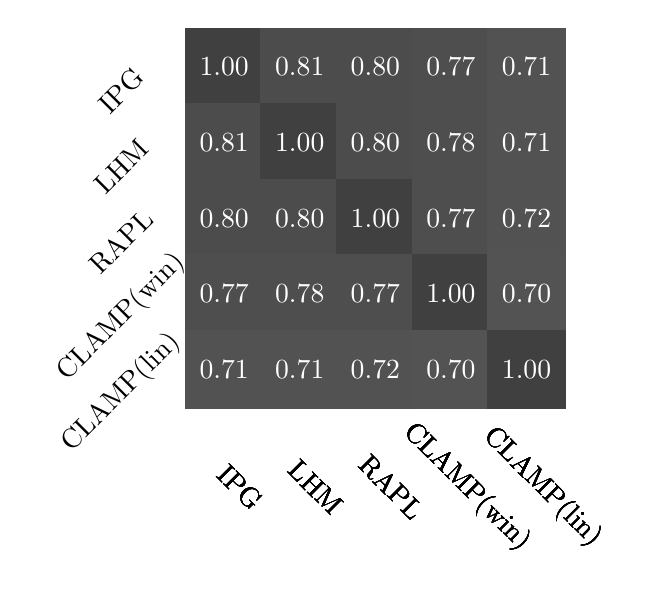
\begin{tikzpicture}[scale=0.6]
  \foreach \y [count=\n] in {{1.00, 0.81, 0.80, 0.77, 0.71},{0.81, 1.00, 0.80, 0.78, 0.71},{0.80, 0.80, 1.00, 0.77, 0.72},{0.77, 0.78, 0.77, 1.00, 0.70},{0.71, 0.71, 0.72, 0.70, 1.00},} {
  % column labels
  \foreach \a [count=\n] in {IPG,LHM,RAPL,CLAMP(win),CLAMP(lin)} {
    \node[minimum size=10mm, xshift=0.2cm, rotate=-45] at (\n*1.6, -10.50) {\a};
  }
  % heatmap tiles
  \foreach \x [count=\m] in \y {
    \pgfmathsetmacro{\xa }{(\x + 1) / 2 * 100}
    \node[fill=darkgray!\xa!lightgray, minimum size=10mm, text=white, font={\normalsize}] at (\m*1.6,-\n*1.6) {\x};
  }
}
  % row labels
  \foreach \a [count=\i] in {IPG,LHM,RAPL,CLAMP(win),CLAMP(lin)} {
    \node[minimum size=10mm, xshift=-0.35cm, yshift=-0.3cm, rotate=45] at (0,-\i*1.6) {\a};
  } 
\end{tikzpicture}
\caption{This heat map represents Correlation coefficients between the different measurement instruments -1 to 1 on the Workstation}
\label{tab:correlationWork}
\end{figure}